\section{REST}

REST (\textit{Representational State Transfer}) é um estilo de arquitetura usada para a comunicação de aplicações distribuídas através do protocolo HTTP. Foi introduzido por Roy Fielding em 2000 com o objetivo de oferecer às aplicações Web um modelo de interface de acesso baseada em recursos. Além disso, descreve seis tipos de restrições que serviços deveriam aplicar para ganho de performance, escalabilidade, simplicidade, modificabilidade, visibilidade, portabilidade e confiabilidade.

Em virtude de causar grande repercussão após sua publicação, o termo REST, segundo Richardson, acabou sofrendo diversas interpretações durante o tempo e sua descrição foi representada de formas não originalmente propostas por Fielding \cite{RichardsonEtAl2013}. Alguns descrevem que serviços que violam essas restrições não podem ser considerados RESTful. Para Wildermuth, apesar de reconhecer as vantagens de cada restrição, serviços Web devem usá-los de forma pragmática. \cite{Wildermuth2015}

Ao ser introduzido no mercado de APIs Web, REST acabou se adaptando bem por ter se mostrado uma solução de fácil acesso em clientes. Segundo Pautasso, a eliminação da complexidade existente em Web Services antes de sua publicação em 2000 fez com que REST fosse considerado um dos principais responsáveis pela popularização de arquiteturas orientada a serviços, visível pela figura 7. \cite{PautassoEtAl2008}

\begin{figure}[H]
  \centering    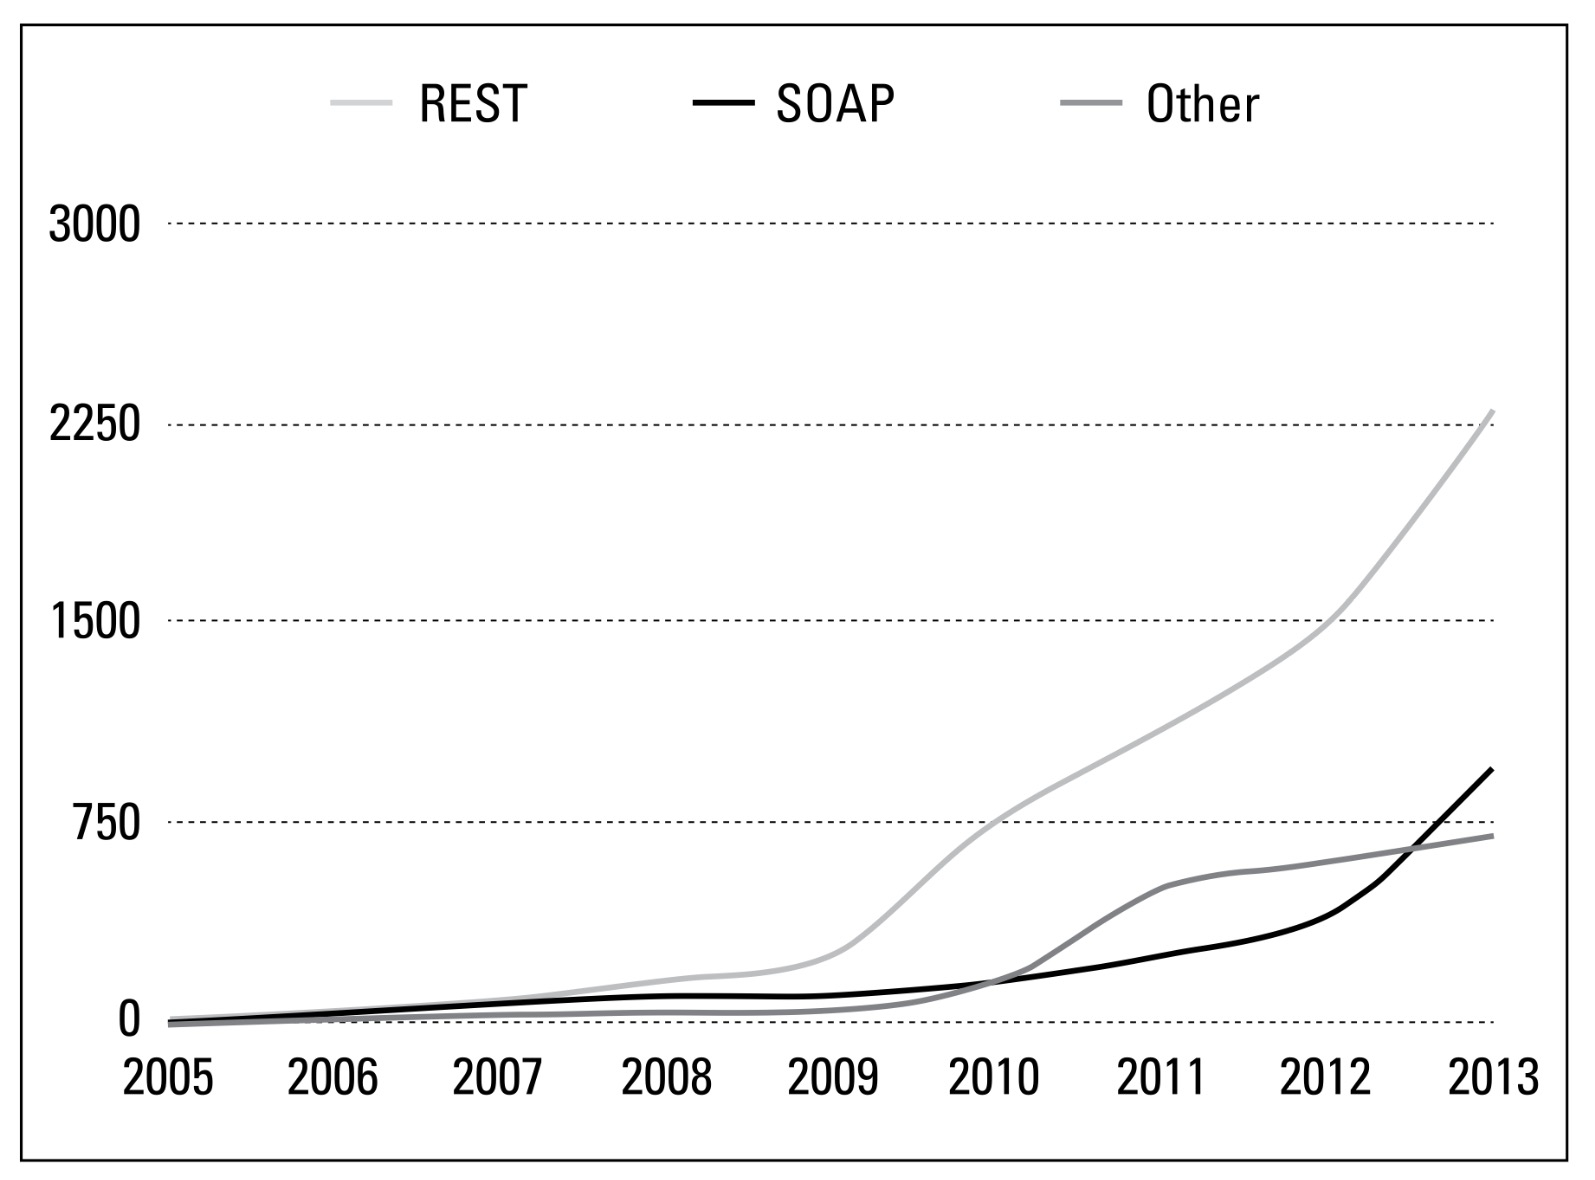
\includegraphics[width=0.9\textwidth,height=\textheight,keepaspectratio]{figuras/api-styles.jpg}
  \caption{Distribuição de estilos e protocolos para APIs Web}
\end{figure}

A seguir será apresentada uma visão geral sobre as restrições propostas por Fielding para a implementação da arquitetura, além de ser examinado o impacto de cada restrição em aplicações distribuídas. \\

\textbf{Cliente-Servidor} \\

Nesta primeira restrição, não existe conexão entre duas aplicações distribuídas, mas sim a espera de uma (servidor) por pedidos da outra (clientes) através de chamada e resposta. O cliente (consumidor do serviço) não se preocupa com tarefas de comunicação de banco de dados, gerenciamento de cache, entre outros. O mesmo ocorre como o servidor (prestador de serviços), que não está preocupado com as tarefas do cliente como interface ou experiência do usuário, por exemplo. Isso permite a evolução independente dos dois ambientes, desde que a interface usada para comunicação entre o cliente e o servidor não seja alterada. \cite{Fielding2000} \\

\textbf{Sem Estado} \\

Esta restrição ajuda na viabilidade, confiabilidade e escalabilidade de aplicações distribuídas, pois garante que chamadas à API não estejam vinculadas a um determinado servidor. Como HTTP é um protocolo sem conexão, cada requisição deve conter todas as informações necessárias para que um servidor entenda o que um cliente está executando. Para Wildermuth, no entanto, dependendo da diversidade no número de clientes, ao manter um servidor sem estado, perder-se o controle no tamanho da estrutura de resposta necessária para atender a demanda de todos os clientes. \cite{Wildermuth2015} \\

\textbf{Interface Uniforme} \\

Em essência, Fielding propõe que aplicações façam o uso de verbos HTTP (POST, GET, PUT, DELETE) e identificadores uniformes de recursos (URIs) para mapear operações em APIs e minimizar o acoplamento na comunicação cliente-servidor. Essas regras de acesso são: \cite{Fielding2000}

\begin{itemize}
\item Identificação de Recursos: Cada recurso deve ser disponibilizado através de uma URI específica e coesa. (Exemplo: GET /customers/1)
\item Manipulação de Recursos através de Representações: Um recurso pode ser representado em diferentes formatos para diferentes clientes. (Exemplo: HTML, XML, JSON)
\item Resposta Auto-explicativa: Metadados devem ser adicionados na requisição e resposta de um recurso para descrever seu estado atual ou desejado. (Exemplo: código de resposta HTTP, Host, Content-Type)
\item HATEOAS (\textit{Hypermedia as the Engine of Application State}): Caso um recurso possua relacionamentos, ao ser representado, estes devem estar especificados em forma de \textit{hyperlinks} para facilitar a navegação de dados por clientes.
\end{itemize}

\textbf{Separação em Camadas} \\

Um dos princípios desta restrição está em evitar que clientes façam diretamente requisição para o servidor sem antes passar por um intermediário, como por exemplo um balanceador de carga (\textit{load balancer})\footnote{
  Técnica para distribuir a carga de trabalho uniformemente entre dois ou mais computadores
}. Desse modo, fica assegurado que clientes apenas se preocupem com a comunicação, deixando que intermediários lidem com a distribuição de requisições. \cite{Fielding2000} \\

\textbf{Código sob Demanda} \\

Apesar de ser a única restrição opcional do estilo, ela permite que servidores disponibilizem código em forma de script para que seja executado no cliente. Dessa forma, a lógica de serviço do servidor é estendida para seus clientes. \cite{Fielding2000} \\

\textbf{Cache} \\

Visa aumentar o desempenho de um serviço. Quando um recurso é acessado por mais de um cliente, se não houve mudança é recomendado que a resposta seja armazenada em cache, evitando o processamento desnecessário. Isso significa que servidores, quando possível, devem implementar regras de cache para beneficio de ambos os ambientes. \cite{Fielding2000}
